O setor de jogos digitais está em expansão, projetando ultrapassar os US\$ 200 bilhões em 2023, conforme previsto por \citeonline{quanto_games_vao_movimentar}. Em 2022, somente na plataforma Steam, foram lançados 10.644 novos títulos, e até 6 de outubro de 2023, 9.103 jogos foram lançados, conforme evidenciado pela Figura 1, que revela uma tendência crescente de lançamentos na Steam ao longo dos anos.

\begin{figure}[!ht]
	\centering
    \caption{Número de jogos publicados na Steam.}
	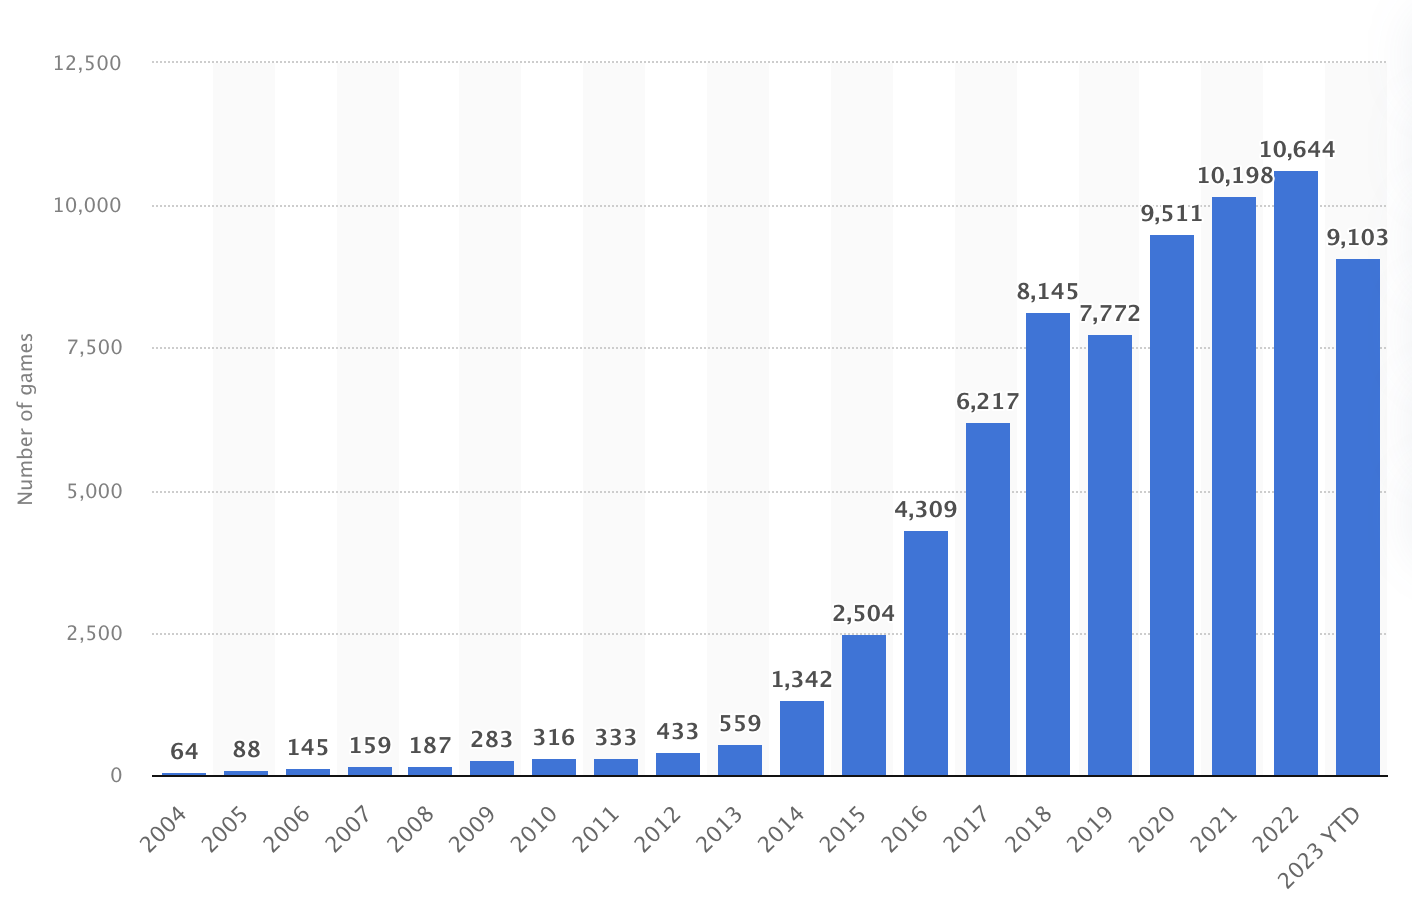
\includegraphics[width=0.6\textwidth]{figures/steam_sales.png}
	\legend{Fonte: \citeonline{numero_de_jogos_publicados_na_steam}}
	\label{fig:steam_publishes}
\end{figure}

Dentro do universo dos jogos, os mapas desempenham um papel crucial, não apenas orientando os jogadores, mas também enriquecendo a experiência ao criar uma sensação de escala e proporcionar uma exploração mais rica \cite{video_game_maps, minimap}.

Na elaboração de mapas, utiliza-se a técnica de geração procedural, baseada na criação dinâmica de conteúdo por meio de algoritmos. Essa abordagem surgiu com o propósito de gerar mapas durante a execução de um programa, minimizando as demandas de armazenamento. Mesmo com a superação das limitações de armazenamento, a geração procedural persiste como uma estratégia para a produção de conteúdos exclusivos a cada execução do programa \cite{kenny2021procedural, lambda3}.

Dentro da geração procedural, diversas técnicas são exploradas, conforme discutido por \citeonline{kvrivzmulti}. Destacam-se o \textit{Perlin Noise}, útil na criação de contornos e texturas naturais, os \textit{L-systems}, empregados na geração de vegetação, o \textit{Voronoi}, utilizado para criar texturas e particionar espaços 2D, e os autômatos celulares, aplicados na criação de cavernas em 2D, entre outras abordagens.

Na geração procedural, surgem desafios, conforme descrito por \citeonline{geracao_procedural_jogos_2d}: "Um dos maiores desafios no desenvolvimento de algoritmos para geração de mapas é a dificuldade de criar cenários que sejam, ao mesmo tempo, atraentes e diversificados, permitindo que o jogador possa explorar um novo ambiente a cada sessão de jogo" \cite{geracao_procedural_jogos_2d}.

Para criar um mapa diversificado, será definido um escopo, tomando como referência o jogo \textit{Minecraft}, que gera mapas proceduralmente com biomas contendo diferentes flora, fauna, relevo, temperaturas, umidade, etc \cite{mojang}. Definido o escopo, um mapa com biomas será gerado utilizando a abordagem proposta por \citeonline{amitp2010}, que utiliza o diagrama de Voronoi para particionar em regiões atribuíveis a diferentes biomas.

Além disso, para adicionar uma camada de personalização e aprimorar a diversidade, será introduzida uma nova funcionalidade que permite definir o contorno do mapa a partir da segmentação de uma foto de um desenho ou de um contexto cotidiano. Para isso, serão utilizadas técnicas de segmentação para classificar a imagem em conjuntos de desenhos, além de técnicas de inteligência artificial (IA) para segmentar cenários mais complexos, os quais podem incluir elementos como pessoas e veículos  \cite{dp_semantic_segmantation, saiwa}.

Portanto, o escopo compreende a geração procedural de mapas com biomas, permitindo a escolha do contorno a partir de um desenho com técnicas de segmentação ou da segmentação de uma imagem mais complexa com modelos de IA. Essa aplicação facultará aos desenvolvedores a incorporação dessa nova funcionalidade em um jogo em fase de desenvolvimento, permitindo ao usuário final a opção de selecionar ou capturar uma foto e escolher um contorno específico para gerar um mapa contendo os biomas.

Por fim, para contribuição científica, a hipótese é que quanto mais pontos o diagrama de Voronoi tiver, maior será a precisão na compatibilidade entre o mapa gerado e o contorno escolhido. Para chegar a essa conclusão, serão realizados testes com métricas para mensurar a qualidade da geração procedural com o contorno selecionado.

\section{Objetivos}

O objetivo principal deste trabalho é desenvolver uma ferramenta que ofereça uma alternativa para a geração procedural de mapas de ilhas, utilizando o diagrama de Voronoi para a criar biomas. Além disso, pretende-se combinar segmentação com redes neurais convolucionais para permitir a personalização desses mapas. Essa ferramenta terá a capacidade de reconhecer os contornos reconhecidos (classificados no conjunto de dados, logo o resultado terá uma detecção abrangente dentro do escopo de classes obtidas) de uma imagem, e gerar um mapa com um mapa baseado nos limites do contorno escolhido.

Adicionalmente, os seguintes objetivos específicos serão abordados:

\begin{itemize}
	\item Selecionar e analisar conjuntos de dados contendo classes relevantes, como pessoas, carros, entre outros, para treinar um modelo de rede neural convolucional específico para segmentação de imagens.
	\item Utilizar algoritmos para criar diagramas de Voronoi.
	\item Aplicar um algoritmo para reconhecer a imagem com o contorno selecionado e gerar como resultado a imagem do mapa gerado.
	\item Utilizar o resultado da segmentação para selecionar indicar o que é terreno em cima do diagrama de Voronoi.
	\item Gerar os biomas no diagrama de Voronoi.
	\item Criar testes em prol de mensurar a semelhança entre o contorno do mapa gerado com o contorno escolhido.
\end{itemize}